\documentclass[table]{beamer}

%\usetheme[secheader]{Boadilla}
\usetheme{Boadilla}
\usecolortheme{beetle}
\usepackage[latin1]{inputenc}
\usepackage{listings} % for code syntax highlighting
\usepackage{caption}

\usepackage{color}
\usepackage{booktabs} % better tables
\usepackage{colortbl} % for coloring tables

%%%%%%%%%%%%%%%%%%%%%%%%%%%%%%%%%%%%%%%%%%%%%%%%%%%%%%%%%%%%%%%%%%%%%%%%%%%
%{{{                               Fonts                                  %
%%%%%%%%%%%%%%%%%%%%%%%%%%%%%%%%%%%%%%%%%%%%%%%%%%%%%%%%%%%%%%%%%%%%%%%%%%%


\usepackage{inconsolata} % for code
\usepackage{lmodern} % normal text
\renewcommand*\familydefault{\sfdefault} 
\usepackage[T1]{fontenc}
%}}}

%%%%%%%%%%%%%%%%%%%%%%%%%%%%%%%%%%%%%%%%%%%%%%%%%%%%%%%%%%%%%%%%%%%%%%%%%%%
%{{{                      Beamer Theme and colors                         %
%%%%%%%%%%%%%%%%%%%%%%%%%%%%%%%%%%%%%%%%%%%%%%%%%%%%%%%%%%%%%%%%%%%%%%%%%%%

 
\definecolor{themegray}{HTML}{999999}
\definecolor{codebg}{HTML}{2C2C2C} % dark gray
\definecolor{codefg}{HTML}{D0D0D0} % light gray
\definecolor{themeblue}{HTML}{789FEF} % light blue
\definecolor{codecomment}{HTML}{808080} % gray
\definecolor{codestring}{HTML}{DFDF87} % for strings, light yellow
\definecolor{themedarkblue}{HTML}{1D2561}
\definecolor{themegreen}{HTML}{6ABF29}
\definecolor{themeyellow}{HTML}{DFDF67}
\definecolor{themeorange}{HTML}{DF8F27}

% tweak beamer theme
\setbeamercolor{framesubtitle}{fg=white}
\setbeamercolor{frametitle}{bg=codebg}
\setbeamercolor{title}{bg=codebg}
\setbeamercolor{palette primary}{bg=themedarkblue}
\setbeamercolor{author}{fg=white}
\setbeamercolor{date}{fg=white}
%}}}

%%%%%%%%%%%%%%%%%%%%%%%%%%%%%%%%%%%%%%%%%%%%%%%%%%%%%%%%%%%%%%%%%%%%%%%%%%%
%{{{                           Tweak Tables                               %
%%%%%%%%%%%%%%%%%%%%%%%%%%%%%%%%%%%%%%%%%%%%%%%%%%%%%%%%%%%%%%%%%%%%%%%%%%%

\setlength{\aboverulesep}{0pt}
\setlength{\belowrulesep}{0pt}
\setlength{\extrarowheight}{.75ex}
%}}}
 
%%%%%%%%%%%%%%%%%%%%%%%%%%%%%%%%%%%%%%%%%%%%%%%%%%%%%%%%%%%%%%%%%%%%%%%%%%%
%{{{                          Tweak Listings                              %
%%%%%%%%%%%%%%%%%%%%%%%%%%%%%%%%%%%%%%%%%%%%%%%%%%%%%%%%%%%%%%%%%%%%%%%%%%%

% caption stuff
\DeclareCaptionFormat{listing}{\parbox{\textwidth}{#1#2#3}}
\captionsetup[lstlisting]{format=listing}

\lstset{ %
  language=C++,                % the language of the code
  basicstyle=\small\ttfamily\color{codefg},           % the size of the fonts that are used for the code
  backgroundcolor=\color{codebg},      % choose the background color. You must add \usepackage{color}
  showspaces=false,               % show spaces adding particular underscores
  showstringspaces=false,         % underline spaces within strings
  showtabs=false,                 % show tabs within strings adding particular underscores
  %frame=single,                   % adds a frame around the code
  rulecolor=\color{black},        % if not set, the frame-color may be changed on line-breaks within not-black text (e.g. commens (green here))
  tabsize=2,                      % sets default tabsize to 2 spaces
  captionpos=t,                   % sets the caption-position to bottom
  breaklines=true,                % sets automatic line breaking
  breakatwhitespace=false,        % sets if automatic breaks should only happen at whitespace
  title=\lstname,                   % show the filename of files included with \lstinputlisting;
                                  % also try caption instead of title
  keywordstyle=\color{themeblue}\bfseries,
  stringstyle=\color{codestring},
  commentstyle=\color{codecomment},
  escapeinside={\%*}{*)},            % if you want to add LaTeX within your code
  morekeywords={*,...}               % if you want to add more keywords to the set
}
% ========================================== }}}

%%%%%%%%%%%%%%%%%%%%%%%%%%%%%%%%%%%%%%%%%%%%%%%%%%%%%%%%%%%%%%%%%%%%%%%%%%%
%{{{                  Custom Macros for Presentation                      %
%%%%%%%%%%%%%%%%%%%%%%%%%%%%%%%%%%%%%%%%%%%%%%%%%%%%%%%%%%%%%%%%%%%%%%%%%%%

% define a counter for rules
\newcounter{rulecount}
\newcommand{\declarerule}{\textbf{\color{themeblue}{Rule \therulecount:}} }

\newcommand{\declarelesson}{\textbf{\color{themegreen}{Lesson:}} }

% behind the scenes title
\newcommand{\declarebts}{\textbf{\color{themeorange}{Behind the Scenes:}} }
%}}}

%%%%%%%%%%%%%%%%%%%%%%%%%%%%%%%%%%%%%%%%%%%%%%%%%%%%%%%%%%%%%%%%%%%%%%%%%%%
%{{{                            Author info                               %
%%%%%%%%%%%%%%%%%%%%%%%%%%%%%%%%%%%%%%%%%%%%%%%%%%%%%%%%%%%%%%%%%%%%%%%%%%%


\title{Forgetting the C in C++}
\author{Alexander Kondratskiy}
\date{\today}
% \institute[2008]{ECON 101}

%}}}

%%%%%%%%%%%%%%%%%%%%%%%%%%%%%%%%%%%%%%%%%%%%%%%%%%%%%%%%%%%%%%%%%%%%%%%%%%%
%{{{                         Main Presentation                            %
%%%%%%%%%%%%%%%%%%%%%%%%%%%%%%%%%%%%%%%%%%%%%%%%%%%%%%%%%%%%%%%%%%%%%%%%%%%


\begin{document}

\frame{\titlepage}

\section{Introduction}
\frame{\sectionpage}

\frame {
    \frametitle{What is the talk about?}
    \begin{itemize}
        \item<2->Overview of C++, from a C programmer's perspective
        \item<2->Good C++ coding style
        \item<2->More than "C with classes"
        \item<2->Fixing bad habbits learnt from C.
    \end{itemize}
}

% Misinformation
\frame {
    \frametitle{Motivation}
    \begin{itemize}
        \item Wealth of misinformation on the internet about C++
        \item The name C++ gives the wrong (and lasting) first impression
        \item Most code examples could have come from 1985
        \item A language is not just its syntax
        \begin{itemize}
            \item Collective experience provides idioms
        \end{itemize}
    \end{itemize}
}

% Buzzwords
\frame {
    \frametitle{Motivation}
    \begin{itemize}
        \item<1->C++ has evolved
        \item<2->\alert{Safety}/Robustness
            \begin{itemize}
                \item Compiler checks
                \item Resource management (including memory)
                \item Type safety
            \end{itemize}
        \item<2->\alert{Readability}/Maintainability
            \begin{exampleblock}{}
                ``Programs must be written for people to read, and only incidentally for machines to execute.''
                \hspace*\fill{\small--- Abelson/Sussman, SICP}
            \end{exampleblock}
        \item<2->Programmer \alert{Productivity}
            \begin{itemize}
                \item STL
                \item Abstractions
            \end{itemize}
        \item<2->\alert{Efficiency} and speed
            \begin{itemize}
                \item More context for compiler
            \end{itemize}
        \item<3->Win-win
    \end{itemize}
}

% Guiding Principles
%\begin{frame}
    %\frametitle{Motivation}
    %\framesubtitle{Guiding Principles}
    %% TODO: move to STL?
    %\begin{exampleblock}{}
        %``If I have seen further, it is by standing on the shoulders of giants''

        %\hspace*\fill{\small--- Isaac Newton}
    %\end{exampleblock}

    %\begin{exampleblock}{}
        %``Make interfaces easy to use correctly and hard to use incorrectly''

        %\hspace*\fill{\small--- Scott Meyers}
    %\end{exampleblock}

%\end{frame}

\begin{frame}
    \frametitle{Method}
    \begin{itemize}
        \item<1->Observe common C idiom
        \item<1->Discuss disadvantages
        \item<1->C++ alternative
        \item<1->Gains from the alternative
        \item<2->Learn new techniques/features along the way
    \end{itemize}
\end{frame}
%}}}

%%%%%%%%%%%%%%%%%%%%%%%%%%%%%%%%%%%%%%%%%%%%%%%%%%%%%%%%%%%%%%%%%%%%%%%%%%%
%{{{                           Prerequisites                              %
%%%%%%%%%%%%%%%%%%%%%%%%%%%%%%%%%%%%%%%%%%%%%%%%%%%%%%%%%%%%%%%%%%%%%%%%%%%

\section{Prerequisites}
\frame{\sectionpage}

\begin{frame}
    \frametitle{\declarelesson History of C++}
    \begin{columns}[t]
        \column{7cm}
        \begin{itemize}
            \item<1->Started by Bjarne Stroustrup in 1979 as "C with Classes"
                \begin{itemize}
                    \item At Bell labs
                    \item "Down the hall" from Dennis Ritchie (creator of C)
                \end{itemize}
            \item<1->Renamed to C++ in 1983, commercially implemented in 1985
            \item<2->1990s: stream IO, STL, ISO Standard in 98
            \item<3->2000s: Boost, TR1 in 2007
            \item<4->2010s: C++11 in 2011
        \end{itemize}
        \column[T]{4cm}
        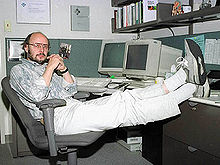
\includegraphics[width=4cm]{220px-BjarneStroustrup.jpg}
    \end{columns}
\end{frame}

%}}}

%%%%%%%%%%%%%%%%%%%%%%%%%%%%%%%%%%%%%%%%%%%%%%%%%%%%%%%%%%%%%%%%%%%%%%%%%%%
%{{{                            Compilation                               %
%%%%%%%%%%%%%%%%%%%%%%%%%%%%%%%%%%%%%%%%%%%%%%%%%%%%%%%%%%%%%%%%%%%%%%%%%%%

\subsection{Compilation}
\frame{\subsectionpage}

% C Compilation
\begin{frame}
    \frametitle{\declarelesson C Compilation model}
    \framesubtitle{A single source file}
    \begin{columns}[t]
        \column{4cm}
        \begin{itemize}
            \item One source file at a time
            \item Preprocessor \emph{resolves all directives}
            \item Compiled to an object file
            \item Missing external function definitions
        \end{itemize}
        \column[T]{8cm}
        \includegraphics[height=9cm,angle=-90]{diagrams/c_compilation_model.pdf}
    \end{columns}
\end{frame}

% Linker
\begin{frame}
    \frametitle{\declarelesson C Compilation model}
    \framesubtitle{Linking}
    \begin{columns}[t]
        \column{4cm}
        \begin{itemize}
            \item Linker combines several translation units
            \item Resolves external dependencies
        \end{itemize}
        \column[T]{8cm}
        \includegraphics[height=9cm,angle=-90]{diagrams/c_compilation_model_linker.pdf}
    \end{columns}
\end{frame}

% Linker + Compiler large diagram
\begin{frame}
    \frametitle{\declarelesson C Compilation model}
    \framesubtitle{A typical project}
    \includegraphics[height=12cm,angle=-90]{diagrams/c_compilation_model_2.pdf}
\end{frame}

\begin{frame}
    \frametitle{\declarelesson C++ Compilation model}
    \begin{itemize}
        \item Same as C compilation model
        \item Template instantiation happens in the compiler
    \end{itemize}
\end{frame}
%}}}

%%%%%%%%%%%%%%%%%%%%%%%%%%%%%%%%%%%%%%%%%%%%%%%%%%%%%%%%%%%%%%%%%%%%%%%%%%%
%{{{                               Scope                                  %
%%%%%%%%%%%%%%%%%%%%%%%%%%%%%%%%%%%%%%%%%%%%%%%%%%%%%%%%%%%%%%%%%%%%%%%%%%%

\subsection{Scope}
\frame{\subsectionpage}

\begin{frame}[fragile]
    \frametitle{\declarelesson Scope}
    \begin{lstlisting}[basicstyle=\scriptsize\ttfamily\color{codefg}]
int globalVar;

namespace SomeNamespace {
    int namespaceVar;

    class SomeClass {
        static int classVar;

        int instanceVar; // aka member variable

        void someMethod() {
            int methodVar;

            if (someCondition) {
                int localVar;
            }
        }
    }
}
    \end{lstlisting}
\end{frame}

\begin{frame}
    \frametitle{\declarelesson Scope}

    \rowcolors{2}{codecomment}{themegray}
    \begin{table}[tl]
        \begin{tabular}{p{3cm}p{2.5cm}p{2.5cm}}
            \rowcolor{codebg}
            \color{white} Variable & \color{white} Lifetime & \color{white} Lexical Scope\\
                          global & global & global \\
                       namespace & global & namespace \\
                        class & global & class \\
                     instance & instance & class \\
                     method / function & function & function \\
                     block & block & block \\
        \end{tabular}
    \end{table}
    \begin{itemize}
        \item Concepts of \emph{lifetime} and \emph{lexical scope} are important
    \end{itemize}
\end{frame}

% TODO: :: syntax for accessing

%}}}

%%%%%%%%%%%%%%%%%%%%%%%%%%%%%%%%%%%%%%%%%%%%%%%%%%%%%%%%%%%%%%%%%%%%%%%%%%%
%{{{                    Local Variable Declaration                        %
%%%%%%%%%%%%%%%%%%%%%%%%%%%%%%%%%%%%%%%%%%%%%%%%%%%%%%%%%%%%%%%%%%%%%%%%%%%

% C variable declaration
\stepcounter{rulecount}
\begin{frame}[fragile]
    \frametitle{\declarerule Declare variables locally}
    \begin{lstlisting}[title=In ANSI C variables must be declared at the beginning of scope]
int someFunc() {
    struct Foo foo;
    struct Bar bar;
    /* ... another 15 declarations */

    /* 
     * use foo.
     * more lines of code
     */

    /* 
     * start using bar
     */
 }
    \end{lstlisting}
\end{frame}

% Local variable declaration C++
\begin{frame}[fragile]
    \frametitle{\declarerule Declare variables locally}
    \begin{lstlisting}[title=In C++ variables can be declared in the middle of scope where they are used]
int someFunc() {
    struct Foo foo;
    // use foo

    struct Bar bar;
    // use bar

    // ...
 }
    \end{lstlisting}
    \begin{itemize}
        \item Declares intent to reader and compiler
            \begin{itemize}
                \item \alert{Readability}
                \item \alert{Efficiency} (compiler optimization)
            \end{itemize}
        \item Reduces variable scope
            \begin{itemize}
                \item less potential for error
            \end{itemize}
    \end{itemize}
\end{frame}
%}}}

%%%%%%%%%%%%%%%%%%%%%%%%%%%%%%%%%%%%%%%%%%%%%%%%%%%%%%%%%%%%%%%%%%%%%%%%%%%
%{{{                      Pointers vs References                          %
%%%%%%%%%%%%%%%%%%%%%%%%%%%%%%%%%%%%%%%%%%%%%%%%%%%%%%%%%%%%%%%%%%%%%%%%%%%

\subsection{Pointers and References}
\frame{\subsectionpage}

% Pointer description
\begin{frame}
    \frametitle{\declarelesson Pointers and References}
    \framesubtitle{Pointers *}
    \begin{itemize}
        \item Pointers are useful
            \begin{itemize}
                \item Refer to a place in memory
                \item Can represent an array
                \item Can create complex data structures
                \item Lightweight way to pass large objects
            \end{itemize}
        \item Pointers are dangerous
            \begin{itemize}
                \item Value unrestricted
                \item Memory management
                \item Pointer arithmetic tricky
            \end{itemize}
    \end{itemize}
\end{frame}

% Pointer usage
\begin{frame}[fragile]
    \frametitle{\declarelesson Pointers and References}
    \framesubtitle{Pointers *}
    \begin{lstlisting}[title=Pointer Usage]
struct Foo {
    int a;
    int b;
}

Foo myFoo;

Foo* pFoo;              // uninitialized pointer

pFoo = &myFoo;          // pointing to an object

Foo anotherFoo = *pFoo; // dereferencing

pFoo->a = 42;           // accessing member
    \end{lstlisting}
\end{frame}

% Reference description
\begin{frame}
    \frametitle{\declarelesson Pointers and References}
    \framesubtitle{References \&}
    \begin{itemize}
        \item References more restricted
            \begin{itemize}
                \item Cannot be \texttt{NULL}
                \item Has to be initialized at creation
                \item Cannot be reassigned
            \end{itemize}
        \item References are safer
            \begin{itemize}
                \item Useful for object passing
                \item Act as an alias to a value
            \end{itemize}
        \item Implemented as a pointer behind the scenes
        \item But usage is restricted at compile time (\alert{Safety})
    \end{itemize}
\end{frame}

% reference usage
\begin{frame}[fragile]
    \frametitle{\declarelesson Pointers and References}
    \framesubtitle{References \&}
    \begin{lstlisting}[title=Reference Usage]
struct Foo {
    int a;
    int b;
}

Foo myFoo;

Foo& aliasFoo = myFoo;     // aliasing a value

Foo anotherFoo = aliasFoo; // copy

aliasFoo.a = 42;           // accessing member
    \end{lstlisting}
\end{frame}

% use in functions
\begin{frame}[fragile]
    \frametitle{\declarelesson Pointers and References}
    \framesubtitle{References \&}
    \begin{lstlisting}[title=Function declaration]
void doSomething(Foo& foo) {
    foo.a = 42;
}
    \end{lstlisting}
    \begin{itemize}
        \item Callee knows object in usable state
            \begin{itemize}
                \item No \texttt{NULL}/error check
            \end{itemize}
    \end{itemize}
    \begin{lstlisting}[title=Function call]
Foo myFoo;

doSomething(myFoo);
    \end{lstlisting}
    \begin{itemize}
        \item Caller knows that function assumes usable state
        \item References declare intent to reader (\alert{Readability})
        \item Compiler enforced (\alert{Safety})
    \end{itemize}
\end{frame}

% Summary
\begin{frame}
    \frametitle{\declarelesson Pointers and References}
    \framesubtitle{Summary}
    \rowcolors{2}{codecomment}{themegray}
    \begin{table}[tl]
        \begin{tabular}{p{4.5cm}p{2.5cm}p{2.5cm}}
            \rowcolor{codebg}
            \color{white} Property & \color{white} Pointer & \color{white}  Reference \\
                       polymorphic & yes & yes \\
              can be \texttt{NULL} & yes & no \\
                 can be reassigned & yes & no \\
                 can uninitialized & yes & no \\
           arithmetic manipulation & yes & no \\
                     member access & -> & . \\
        \end{tabular}
    \end{table}
    \begin{itemize}
        \item When references can be used, each row is one less headache
    \end{itemize}
\end{frame}

% Prefer references
\stepcounter{rulecount}
\begin{frame}
    \frametitle{\declarerule Prefer References to Pointers}
    \fontsize{12pt}{14}\selectfont
    \begin{itemize}
        \item Use \emph{references} always, unless you can't
        \item Use \emph{pointers} when
            \begin{itemize}
    \fontsize{10pt}{11}\selectfont
                \item passing a NULL pointer is valid semantically
                \item requiring pointer arithmetic (e.g. arrays)
                \item dealing with heap allocation
            \end{itemize}
    \end{itemize}
\end{frame}
%}}}

%%%%%%%%%%%%%%%%%%%%%%%%%%%%%%%%%%%%%%%%%%%%%%%%%%%%%%%%%%%%%%%%%%%%%%%%%%%
%{{{                         Const correctness                            %
%%%%%%%%%%%%%%%%%%%%%%%%%%%%%%%%%%%%%%%%%%%%%%%%%%%%%%%%%%%%%%%%%%%%%%%%%%%

\subsection{Const correctness}
\frame{\subsectionpage}

% immutability
\begin{frame}[fragile]
    \frametitle{\declarelesson Const correctness}
    \framesubtitle{Immutability}
    \begin{itemize}
        \item Objects are mutable by default
            \begin{itemize}
                \item Value can be modified
            \end{itemize}
    \end{itemize}
    \begin{lstlisting}[title=Passing mutable object]
void doSomething(Foo& foo) {
    foo.a++;
}
    \end{lstlisting}
    \begin{itemize}
        \item Mutability can be undesirable in some cases
            \begin{itemize}
                \item Want to ensure function call will not modify value
                \item Avoid potential race conditions in concurrent code
            \end{itemize}
        \item Need to express immutability
    \end{itemize}
\end{frame}

% const keyword
\begin{frame}[fragile]
    \frametitle{\declarelesson Const correctness}
    \framesubtitle{\texttt{const} keyword}
    \begin{lstlisting}[title=Variables can be declared \texttt{const}]
// have to be initialized when declared
Foo const myFoo = { 42, 7 }; 

myFoo.a++; // Compilation Error! Cannot modify
    \end{lstlisting}
    \begin{lstlisting}[title=Function declaration]
// promises the value will not be modified
void doSomethingConst(Foo const& foo) {

    foo.a++; // Compilation Error! Cannot modify
}
    \end{lstlisting}
    \begin{itemize}
        \item \texttt{const} tells compiler object cannot be modified
    \end{itemize}
\end{frame}

% const functions
\begin{frame}[fragile]
    \frametitle{\declarelesson Const correctness}
    \framesubtitle{\texttt{const} keyword}
    \begin{lstlisting}[title=Mutable objects can be used as const arguments]
// promises the value will not be modified
void doSomethingConst(Foo const& foo);

Foo myFoo;                  // mutable

doSomethingConst(myFoo);    // works!
    \end{lstlisting}
    \begin{lstlisting}[title=Immutable objects cannot be used as non-const arguments]
// value might be modified
void doSomethingNonConst(Foo& foo);

Foo const myFoo = { 42, 7 }; // immutable

doSomethingNonConst(myFoo);  // Error!
    \end{lstlisting}
\end{frame}

% right to left reading
\begin{frame}[fragile]
    \frametitle{\declarelesson Const correctness}
    \framesubtitle{\texttt{const} keyword}
    \begin{itemize}
        \item Variable declarations can be read from right to left
    \end{itemize}
    \begin{lstlisting}[title=const Pointers and references]
// myFoo is a const Foo
Foo const myFoo; 

// myFoo is a reference to const Foo
Foo const& myFoo; 

// myFoo is a pointer to const Foo
Foo const* myFoo; 

// myFoo is a const pointer to const Foo
Foo const* const myFoo; 

// myFoo is a const pointer to mutable Foo
Foo* const myFoo; 
    \end{lstlisting}
\end{frame}

% Rul about const correctness
\stepcounter{rulecount}
\begin{frame}[fragile]
    \frametitle{\declarerule Follow const correctness}
    \framesubtitle{Resolving ambiguities}
    \begin{itemize}
        \item Const correctness can resolve ambiguities
    \end{itemize}
    \begin{lstlisting}[title=Ambiguous declaration without const]
void parse(File* file, XMLTree* xml);
    \end{lstlisting}
    \begin{itemize}
        \item Are both arguments inputs?
        \item Is one an output?
        \item Are any arguments optional? (previous rule)
    \end{itemize}
    \begin{lstlisting}[title=Const correct]
void parse(File const& file, XMLTree& xml);
    \end{lstlisting}
    \begin{itemize}
        \item Apparent that \texttt{file} is only read.
        \item \texttt{xml} is modified using data from \texttt{file}
    \end{itemize}
\end{frame}

% const correct summary
\begin{frame}[fragile]
    \frametitle{\declarerule Follow const correctness}
    \framesubtitle{Summary}
    \begin{itemize}
        \item Use \texttt{const} everywhere you can
        \item Declares intent to the reader (\alert{Readability})
            \begin{itemize}
                \item Code is self documenting
                \item Easier to reason about code functionality
                \item Easier to reason about code correctness
            \end{itemize}
        \item Const correctness enforced by the compiler (\alert{Safety})
    \end{itemize}
\end{frame}
%}}}

%%%%%%%%%%%%%%%%%%%%%%%%%%%%%%%%%%%%%%%%%%%%%%%%%%%%%%%%%%%%%%%%%%%%%%%%%%%
%{{{                           Preprocessor                               %
%%%%%%%%%%%%%%%%%%%%%%%%%%%%%%%%%%%%%%%%%%%%%%%%%%%%%%%%%%%%%%%%%%%%%%%%%%%

\section{Preprocessor}
\frame{\sectionpage}

\stepcounter{rulecount}
\begin{frame}
    \frametitle{\declarerule Avoid the preprocessor}
    \begin{itemize}
        \item Macros are text substitution
        \item Macros not subject to scope rules
        \item Compiler does not see any preprocessor directives only final result of substitution
            \begin{itemize}
                \item No meaningful error checking!
            \end{itemize}
        \item Used naively can lead to subtle, hard to find bugs
    \end{itemize}
\end{frame}

\stepcounter{rulecount}
\begin{frame}[fragile]
    \frametitle{\declarerule Prefer \texttt{const} variables over \texttt{\#define}}
    \framesubtitle{Declaring constants}
\begin{lstlisting}
#define DAYSINWEEK 7
const unsigned int days_in_a_week = 7;
\end{lstlisting}
    \begin{itemize}
        \item Typesafe
            \begin{itemize}
                \item Unambiguous function overload usage
            \end{itemize}
        \item Debugging symbol exists
        \item Scoped
        \item Const variables can be any C++ type, not just numbers
            \begin{itemize}
                \item Can be pointed to
            \end{itemize}
    \end{itemize}
\end{frame}

% Bracketing problem
\stepcounter{rulecount}
\begin{frame}[fragile]
    \frametitle{\declarerule Avoid macro functions}
\begin{uncoverenv}<1->
\begin{lstlisting}[title=Given an innocent macro definition]
#define CIRCLE_AREA(R) 3.14 * R * R
\end{lstlisting}
\end{uncoverenv}

\begin{uncoverenv}<2->
\begin{lstlisting}[title=You write]
double total_area = 2 * CIRCLE_AREA( a + b );
\end{lstlisting}
\end{uncoverenv}

\begin{uncoverenv}<3->
\begin{lstlisting}[title=The compiler sees]
double total_area = 2 * 3.14 * a + b * a + b;
\end{lstlisting}
\begin{itemize}
    \item This code compiles with no errors,
        but is clearly not what is intended
\end{itemize}
\end{uncoverenv}

\end{frame}

% Fixing macro problem with brackets
\begin{frame}[fragile]
    \frametitle{\declarerule Avoid macro functions}
\begin{lstlisting}[title=\textbf{Macro Solution:} Wrap everything in brackets]
#define CIRCLE_AREA(R) (3.14 * (R) * (R))
\end{lstlisting}
\begin{itemize}
    \item<2->Macro functions do not work as functions
    \item<2->This solution is just a bandaid!
    \item<3->But wait... There's more!
\end{itemize}
\end{frame}

% Demonstrate problem with multiline macros
\begin{frame}[fragile]
    \frametitle{\declarerule Avoid macro functions}
    \framesubtitle{Multiline Macros}
    
\begin{uncoverenv}<1->
\begin{lstlisting}[title=A multiline macro that swaps the values of two variables]
#define SWAP(x, y) \
    tmp = x; \
    x = y; \
    y = tmp
\end{lstlisting}

\begin{lstlisting}[title=You write]
if (z == 0)
    SWAP(x, y);
\end{lstlisting}
\end{uncoverenv}

\begin{uncoverenv}<2->
\begin{lstlisting}[title=The compiler sees]
if (z == 0)
    tmp = x;
x = y;
y = tmp;
\end{lstlisting}
\end{uncoverenv}
\end{frame}

% Fix multiline with do while
\begin{frame}[fragile]
    \frametitle{\declarerule Avoid macro functions}
    \framesubtitle{Multiline Macros}
    
    \begin{lstlisting}[title=\textbf{Bandaid solution:} wrap in do-while]
#define SWAP(x, y) \
    do { \
        tmp = x; \
        x = y; \
        y = tmp; \
    } while (0)
\end{lstlisting}
\begin{itemize}
    \item Surely we can get by with bandaids!
\end{itemize}
\end{frame}

% Fix multiline with do while
\begin{frame}[fragile]
    \frametitle{\declarerule Avoid macro functions}
    \framesubtitle{Undefined Behaviour}
    
\begin{uncoverenv}<1->
\begin{lstlisting}[title=A simple abs macro]
#define ABS(x) (((x) < 0) ? -(x) : (x))
\end{lstlisting}

\begin{lstlisting}[title=You write]
m = ABS(++n); 
\end{lstlisting}
\end{uncoverenv}

\begin{uncoverenv}<2->
\begin{lstlisting}[title=The compiler sees]
m = (((++n) < 0) ? -(++n) : (++n));
/* undefined behaviour */
\end{lstlisting}
    \begin{itemize}
        \item Cannot modify object more than once in an expression.
        \item We've run out of bandaids!
    \end{itemize}
\end{uncoverenv}
\end{frame}

% Show solution to macro woes
\begin{frame}[fragile]
    \frametitle{\declarerule Avoid macro functions}
    \framesubtitle{Use inline functions}
\begin{lstlisting}[title=\textbf{Better solution:} inline functions]
inline double circle_area(double radius) {
    return 3.14 * radius * radius;
}
\end{lstlisting}

\begin{lstlisting}
inline void swap(int& x, int& y) {
    int temp = x;
    x = y;
    y = temp;
}
\end{lstlisting}

\begin{lstlisting}
inline double abs(double radius) {
    return (x < 0) ? -x : x;
}
\end{lstlisting}

\end{frame}

% Advantages of inline functions over macros
\begin{frame}[fragile]
    \frametitle{\declarerule Avoid macro functions}
    \framesubtitle{Use inline functions}
    \begin{itemize}
        \item<1->Use inline functions!
            \begin{itemize}
                \item Type safe
                \item Efficient- inlined by compiler
                \item Checked by compiler
                \item Scoped
                \item Can be used in C too
            \end{itemize}
        \item<2->Can we make them type-generic, like macros?
    \end{itemize}
\end{frame}

% Template inline functions
\begin{frame}[fragile]
    \frametitle{\declarerule Avoid macro functions}
    \framesubtitle{C++ to the rescue: templates!}
\begin{lstlisting}
template <typename T>
inline void swap(T& x, T& y) {
    T temp = x;
    x = y;
    y = temp;
}
\end{lstlisting}

\begin{lstlisting}
template <typename T>
inline T abs(T radius) {
    return (x < 0) ? -x : x);
}
\end{lstlisting}
\begin{itemize}
    \item All the advantages of functions
    \item Plus type-generic
\end{itemize}
\end{frame}
%}}}

%%%%%%%%%%%%%%%%%%%%%%%%%%%%%%%%%%%%%%%%%%%%%%%%%%%%%%%%%%%%%%%%%%%%%%%%%%%
%{{{                              Classes                                 %
%%%%%%%%%%%%%%%%%%%%%%%%%%%%%%%%%%%%%%%%%%%%%%%%%%%%%%%%%%%%%%%%%%%%%%%%%%%

\section{Classes}
\frame{\sectionpage}

% Class intro
\begin{frame}[fragile]
    \frametitle{\declarelesson Classes }
    \framesubtitle{Structures in C}
    \begin{lstlisting}[title=Data in C is usually represented with \texttt{struct}s]
struct Mansion {
    int floors;
    int roomsPerFloor;
    struct FloorPlan* floorPlans;
};
    \end{lstlisting}
    \begin{itemize}
        \item Useful for describing aggregate concepts
        \item All data accessible by any function
        \item POD (Plain Old Data)
    \end{itemize}
\end{frame}

% Overview of new features Classes
\begin{frame}
    \frametitle{\declarelesson Classes }
    \framesubtitle{C++ additions}
    \begin{itemize}
        \item C++ introduces classes, which can have ...
            \begin{itemize}
                \item Private and protected members
                \item Constructors
                \item Destructors
                \item Methods
                \item Operators
                \item Inheritance
                \item Virtual methods
                \item Virtual inheritance
            \end{itemize}
        \item Structs can also have all of the above
        \item The \emph{only} difference between structs and classes is
            \begin{itemize}
                \item Classes: \emph{access private} by default
                \item Structs: \emph{access public} by default
            \end{itemize}
    \end{itemize}
\end{frame}
%}}}

%%%%%%%%%%%%%%%%%%%%%%%%%%%%%%%%%%%%%%%%%%%%%%%%%%%%%%%%%%%%%%%%%%%%%%%%%%%
%{{{                           Member access                              %
%%%%%%%%%%%%%%%%%%%%%%%%%%%%%%%%%%%%%%%%%%%%%%%%%%%%%%%%%%%%%%%%%%%%%%%%%%%

% C++ private members
\begin{frame}[fragile]
    \frametitle{\declarelesson Classes }
    \framesubtitle{Private members}
    \begin{itemize}
        \item C++ introduces private members
    \end{itemize}
    \begin{lstlisting}[title=Functions cannot access members]
class Mansion { // members private by default
    int floors;
    int roomsPerFloor;
};

int getTotalRooms(Mansion* mansion) {
    // error!
    return mansion->floors * mansion->roomsPerFloor;
}
    \end{lstlisting}
\end{frame}

% member access errors
\begin{frame}[fragile]
    \frametitle{\declarelesson Classes }
    \framesubtitle{Private members}
    \begin{lstlisting}[title=Compilation errors,basicstyle=\scriptsize\ttfamily\color{codefg},language=bash]
mansion.cpp: In function `int getTotalRooms(Mansion*)':
mansion.cpp:11:9: error: `int Mansion::floors' is private
mansion.cpp:16:21: error: within this context
mansion.cpp:12:9: error: `int Mansion::roomsPerFloor' is private
mansion.cpp:16:39: error: within this context
    \end{lstlisting}
\end{frame}


% C++ access
\begin{frame}[fragile]
    \frametitle{\declarelesson Classes }
    \framesubtitle{Private members}
    \begin{lstlisting}[title=Keywords for defining member access]
class Mansion {
private: // default access in classes
    int floors;
    int roomsPerFloor;

public: // default access in structs
    Address address;

protected: // private, accessible by derived classes
    Plumbing pipes;
};
    \end{lstlisting}
    \begin{itemize}
        \item How can we access private members?
        \item Private members only accessible inside class methods
    \end{itemize}
\end{frame}
%}}}

%%%%%%%%%%%%%%%%%%%%%%%%%%%%%%%%%%%%%%%%%%%%%%%%%%%%%%%%%%%%%%%%%%%%%%%%%%%
%{{{                              Methods                                 %
%%%%%%%%%%%%%%%%%%%%%%%%%%%%%%%%%%%%%%%%%%%%%%%%%%%%%%%%%%%%%%%%%%%%%%%%%%%

\subsection{Methods}
\frame{\subsectionpage}

% Class methods
\begin{frame}[fragile]
    \frametitle{\declarelesson Classes }
    \framesubtitle{Methods}
    \begin{itemize}
        \item Classes can have methods a.k.a. member functions
        \item Can access all members of an object (class instance)
        \item Via implicit \texttt{this} pointer that refers to the object
        \item Can be private, public, and protected 
    \end{itemize}
    \begin{lstlisting}[title=Writing a method]
class Mansion {
    int floors;
    int roomsPerFloor;

public:
    int getTotalRooms() {
        return this->floors * this->roomsPerFloor;
    }
};
    \end{lstlisting}
\end{frame}

% this optional
\begin{frame}[fragile]
    \frametitle{\declarelesson Classes }
    \framesubtitle{Methods}
    \begin{itemize}
        \item implicit \texttt{this} pointer is optional
    \end{itemize}
    \begin{lstlisting}[title=Equivalent]
class Mansion {
public:
    int getTotalRooms() {
        return this->floors * this->roomsPerFloor;
    }

    int getTotalRooms() {
        return floors * roomsPerFloor;
    }
};
    \end{lstlisting}
\end{frame}

% Method usage
\begin{frame}[fragile]
    \frametitle{\declarelesson Classes }
    \framesubtitle{Methods}
    \begin{lstlisting}[title=Using a method]
class Mansion {
public:
    int getTotalRooms() {
        return this->floors * this->roomsPerFloor;
    }
};

Mansion myMansion;
Mansion* mansionPointer;

int total = myMansion.getTotalRooms();
total = mansionPointer->getTotalRooms();
    \end{lstlisting}
    \begin{itemize}
        \item By combining private members and methods, we encapsulate and
            abstract implementation details.
    \end{itemize}
\end{frame}

% Methods and "this" C idiom
\begin{frame}[fragile]
    \frametitle{\declarebts Methods }
    \begin{lstlisting}[title=\texttt{this} pointer idiom in C]
int getTotalRooms(Mansion* this) {
    return this->floors * this->roomsPerFloor;
}
    \end{lstlisting}
    \begin{itemize}
        \item Gives insight into how methods are implemented
    \end{itemize}
    \begin{lstlisting}[title=Calling an object's method]
int total = mansionPointer->getTotalRooms();
    \end{lstlisting}
    \begin{lstlisting}[title=Behind the scenes]
int total = getTotalRooms(mansionPointer);
    \end{lstlisting}
    \begin{itemize}
        \item Methods stored just as functions in final executable (once)
        \item Separate from object's members
        \item Methods work as functions acting on objects
    \end{itemize}
\end{frame}

%TODO: const methods?

%TODO: diagram of methods in memory?

%}}}

%%%%%%%%%%%%%%%%%%%%%%%%%%%%%%%%%%%%%%%%%%%%%%%%%%%%%%%%%%%%%%%%%%%%%%%%%%%
%{{{                           Constructors                               %
%%%%%%%%%%%%%%%%%%%%%%%%%%%%%%%%%%%%%%%%%%%%%%%%%%%%%%%%%%%%%%%%%%%%%%%%%%%

\subsection{Constructors}
\frame{\subsectionpage}

% Introduction to constructors
\begin{frame}[fragile]
    \frametitle{\declarelesson Classes }
    \framesubtitle{Constructors}
    \begin{itemize}
        \item Members have to be initialized on creation (esp. if private)
        \item C++ provides constructors for initialization
        \item A "method" named the same as the class
        \item Members can be initialized in initialization list
    \end{itemize}
    \begin{lstlisting}[title=Default Constructor]
class Mansion {
    int floors;
    int roomsPerFloor;

public:
    Mansion() : floors(3), roomsPerFloor(7) { }
};

Mansion defaultMansion; // 3 floors, 7 rooms per floor
Mansion* heapMansion = new Mansion;
    \end{lstlisting}
\end{frame}

% constructor with arguments
\begin{frame}[fragile]
    \frametitle{\declarelesson Classes }
    \framesubtitle{Constructors}
    \begin{itemize}
        \item Constructors can have arguments
        \item As many constructors as you want (overloading)
    \end{itemize}
    \begin{lstlisting}[title=Constructor with arguments]
class Mansion {
public:
    Mansion() : floors(3), roomsPerFloor(7) { }
    Mansion(int f, int totalRooms)
        : floors(f),
          roomsPerFloor(totalRooms/floors) { }
};

// 3 floors, 7 rooms per floor
Mansion defaultMansion; 
// 2 floors, 5 rooms per floor
Mansion customMansion(2, 10); 
    \end{lstlisting}
\end{frame}
%}}}

%%%%%%%%%%%%%%%%%%%%%%%%%%%%%%%%%%%%%%%%%%%%%%%%%%%%%%%%%%%%%%%%%%%%%%%%%%%
%{{{                         Copy Constructor                             %
%%%%%%%%%%%%%%%%%%%%%%%%%%%%%%%%%%%%%%%%%%%%%%%%%%%%%%%%%%%%%%%%%%%%%%%%%%%

\begin{frame}[fragile]
    \frametitle{\declarelesson Classes }
    \framesubtitle{Copy Constructor}
    \begin{itemize}
        \item Objects can be copied
        \item Need to preserve inner state, and resources
        \item Use copy constructor
    \end{itemize}
    \begin{lstlisting}[title=Copy Constructor]
class Car {
    Wheel* wheel; // unique wheel per car

public:
    Car(Car const& other)
        : wheel(new Wheel(other.wheel)) { }
};

Car myCar;
Car copy(myCar); // calls copy constructor
Car anotherCopy = myCar; // also calls copy constructor
    \end{lstlisting}
\end{frame}

\stepcounter{rulecount}
\begin{frame}[fragile]
    \frametitle{\declarerule Define Copy Constructors }
    \framesubtitle{When necessary}
    \begin{itemize}
        \item Compiler implicitly generates copy constructor when no explicit one exists
        \item Compiler copy constructor blindly copies values
            \begin{itemize}
                \item OK for POD and value aggregates
                \item Bad for objects with pointer members
                \item Bad for objects with state
            \end{itemize}
    \end{itemize}
    \begin{lstlisting}[title=Copy Constructor]
class Car {
    Wheel* wheel;
    // no user copy constructor
    // compiler generates "blind copy" constructor
};

Car myCar;
Car copy(myCar); // calls copy constructor
// myCar and copy share the same wheel
    \end{lstlisting}
\end{frame}

\begin{frame}[fragile]
    \frametitle{\declarerule Define Copy Constructors }
    \framesubtitle{Summary}
    \begin{itemize}
        \item Forgetting to explicitly define a copy constructor 
            changes class semantics
        \item Define your own copy constructor when
            \begin{itemize}
                \item Object has pointer members
                \item Object is a state machine
                \item Creation relies on outside state
                \item ...
            \end{itemize}
        \item Can make copy constructor private to prevent copying
    \end{itemize}
\end{frame}
%}}}

%%%%%%%%%%%%%%%%%%%%%%%%%%%%%%%%%%%%%%%%%%%%%%%%%%%%%%%%%%%%%%%%%%%%%%%%%%%
%{{{                       Initialization lists                           %
%%%%%%%%%%%%%%%%%%%%%%%%%%%%%%%%%%%%%%%%%%%%%%%%%%%%%%%%%%%%%%%%%%%%%%%%%%%

% effect on memory initialization
\stepcounter{rulecount}
\begin{frame}[fragile]
    \frametitle{\declarerule Prefer initialization lists}
    \framesubtitle{In Constructors}
    % TODO: animate?
    \begin{itemize}
        \item Objects not in initialization list are default initialized
    \end{itemize}
    \begin{lstlisting}[title=Assignment in constructor]
class Client {
    Socket sock;

public:
    Client(IPAddress host) {
        sock = Socket(host);
    }
};
    \end{lstlisting}
    \begin{itemize}
        \item Default constructor is called for \texttt{sock} member
        \item Temporary \texttt{Socket} object constructed from \texttt{host}
        \item Assignment operator called to copy temporary into \texttt{sock}
        \item Temporary is destroyed
    \end{itemize}
\end{frame}

\begin{frame}[fragile]
    \frametitle{\declarerule Prefer initialization lists}
    \begin{lstlisting}[title=Initialization list]
class Client {
    Socket sock;

public:
    Client(IPAddress host) : sock(host) { }
};
    \end{lstlisting}
    \begin{itemize}
        \item \texttt{sock} constructed from \texttt{host}
    \end{itemize}
\end{frame}

\begin{frame}
    \frametitle{\declarerule Prefer initialization lists}
    \framesubtitle{Summary}
    \begin{itemize}
        \item Efficient for objects
        \item All initialization in one place (\alert{readability})
    \end{itemize}
\end{frame}
%}}}

%%%%%%%%%%%%%%%%%%%%%%%%%%%%%%%%%%%%%%%%%%%%%%%%%%%%%%%%%%%%%%%%%%%%%%%%%%%
%{{{                            Destructors                               %
%%%%%%%%%%%%%%%%%%%%%%%%%%%%%%%%%%%%%%%%%%%%%%%%%%%%%%%%%%%%%%%%%%%%%%%%%%%

\subsection{Destructors}
\frame{\subsectionpage}

% destructor overview
\begin{frame}[fragile]
    \frametitle{\declarelesson Classes}
    \framesubtitle{Destructors}
    \begin{itemize}
        \item A "method" 
            \begin{itemize}
                \item Named after class, prefixed by \textasciitilde
                \item Takes no arguments
                \item Called at end of object \emph{lifetime}
                \item Destroys all value members
            \end{itemize}
        \item If no explicit destructor defined, implicit one generated
        \item Used to release resources and clean up state
    \end{itemize}
    \begin{lstlisting}[title=Cleanup in destructor]
class Socket {
public:
    ~Socket() {
        // close socket if it hasn't been already
        this->close();
        // any value member automatically destroyed 
    }
};
    \end{lstlisting}
\end{frame}

% when can an object's lifetime end
\begin{frame}
    \frametitle{\declarelesson Classes}
    \framesubtitle{Destructors}
    \begin{itemize}
        \item When does an object's lifetime end?
            \begin{itemize}
                \item See scope table
            \end{itemize}
        \item Object destroyed at end of scope if allocated statically
            \begin{itemize}
                \item End of block scope
                \item End of function scope
                \item Destruction of parent object
            \end{itemize}
        \item Object destroyed when deleted if allocated on the heap
        \item Pointer members are not deleted!
            \begin{itemize}
                \item The memory for pointer released
                \item The object it is pointing to is not
            \end{itemize}
    \end{itemize}
\end{frame}
%}}}

%%%%%%%%%%%%%%%%%%%%%%%%%%%%%%%%%%%%%%%%%%%%%%%%%%%%%%%%%%%%%%%%%%%%%%%%%%%
%{{{                          New and delete                              %
%%%%%%%%%%%%%%%%%%%%%%%%%%%%%%%%%%%%%%%%%%%%%%%%%%%%%%%%%%%%%%%%%%%%%%%%%%%

\subsection{Heap Allocation}
\frame{\subsectionpage}

% Malloc and Free
\stepcounter{rulecount}
\begin{frame}[fragile]
    \frametitle{\declarerule Use \texttt{new} and \texttt{delete} }
    \begin{itemize}
        \item In C, dynamic allocation is done using \texttt{malloc} and \texttt{free}
            \begin{itemize}
                \item Simply allocates number of bytes
                \item Data uninitialized
            \end{itemize}
    \end{itemize}
    \begin{lstlisting}[title=Dynamically allocating a struct in C]
struct Mansion {
    // definition
};

struct Mansion* myMansion =
    (struct Mansion*)malloc(sizeof(struct Mansion));

myMansion->floors = 3; // initialize inner members

free(myMansion);
    \end{lstlisting}
\end{frame}

% New and Delete
\begin{frame}[fragile]
    \frametitle{\declarerule Use \texttt{new} and \texttt{delete} }
    \framesubtitle{Never \texttt{malloc} and \texttt{free} }
    \begin{itemize}
        \item C++ objects have constructors, destructors, inheritance, virtual methods
            \begin{itemize}
                \item Object creation is complicated
            \end{itemize}
        \item Use \texttt{new} and \texttt{delete} in C++
            \begin{itemize}
                \item Size is known by compiler
                \item Correct type is returned (no casting required)
                \item Memory initialized by class constructor
                \item Works for all types
            \end{itemize}
    \end{itemize}
    \begin{lstlisting}[title=Dynamically allocating an object in C++]
class Mansion {
    // definition
};

// calls default constructor
Mansion* myMansion = new Mansion;
delete myMansion;
    \end{lstlisting}
\end{frame}

% new[] and delete[]
\begin{frame}[fragile]
    \frametitle{\declarerule Use \texttt{new} and \texttt{delete} }
    \framesubtitle{Arrays}
    \begin{itemize}
        \item How about allocating arrays in C++?
        \item Use \texttt{new[]} and \texttt{delete[]} for arrays 
            \begin{itemize}
                \item Size need not be a compile-time constant
            \end{itemize}
    \end{itemize}
    \begin{lstlisting}[title=Dynamically allocating an array of objects in C++]
Mansion richArea[] = new Mansion[largeNumber];
delete[] richArea;
    \end{lstlisting}
\end{frame}
%}}}

%%%%%%%%%%%%%%%%%%%%%%%%%%%%%%%%%%%%%%%%%%%%%%%%%%%%%%%%%%%%%%%%%%%%%%%%%%%
%{{{                         RAII EPIC SAUCE!                             %
%%%%%%%%%%%%%%%%%%%%%%%%%%%%%%%%%%%%%%%%%%%%%%%%%%%%%%%%%%%%%%%%%%%%%%%%%%%

\subsection{RAII resource management}
\frame{\subsectionpage}

% RAII intro
\stepcounter{rulecount}
\begin{frame}
    \frametitle{\declarerule Use RAII}
    \framesubtitle{Resources}
    \begin{itemize}
        \item What is RAII?
            \begin{itemize}
                \item We'll get to that...
            \end{itemize}
        \item A large problem in programming is resource management
            \begin{itemize}
                \item Memory allocation
                \item IO handles
                \item Domain specific resources
            \end{itemize}
        \item Besides core logic, need to manage
            \begin{itemize}
                \item Who allocates a resource
                \item Who releases the resources
            \end{itemize}
        \item Usually error prone
            \begin{itemize}
                \item Forgetting to free a pointer
                \item Forgetting to close a file
            \end{itemize}
    \end{itemize}
\end{frame}

% file handle example
\begin{frame}[fragile]
    \frametitle{\declarerule Use RAII}
    \framesubtitle{Resources in C}
    \begin{lstlisting}[title=Reading a file in C]
void process(const char* filename) {
    FILE* fp = fopen(filename, "r");

    // other code

    fclose(fp);
}
    \end{lstlisting}
    \begin{itemize}
        \item Relies on programmer to remember
        \item In C++ any function can throw an exception
    \end{itemize}
\end{frame}

% file leak
\begin{frame}[fragile]
    \frametitle{\declarerule Use RAII}
    \framesubtitle{Resources in C}
    \begin{lstlisting}[title=Forgetting to close]
void process(const char* filename) {
    FILE* fp = fopen(filename, "r");

    // other code

    // error handling
    if (someCondition) {
        return;
    }

    // more code

    fclose(fp);
}
    \end{lstlisting}
    \begin{itemize}
        \item Whoops!
    \end{itemize}
\end{frame}

% towards RAII
\begin{frame}
    \frametitle{\declarerule Use RAII}
    \framesubtitle{Resources in C}
    \begin{itemize}
        \item In previous situation, need to ensure file closes when exiting function
        \item What is triggered on scope exit?
            \begin{itemize}
                \item Local values are destroyed
            \end{itemize}
        \item Exploit destructor to close the file for us!
        \item That is RAII
            \begin{itemize}
                \item Resource Acquisition Is Initialization
                \item Bjarne admits it's a bad name :P
            \end{itemize}
        \item Let's do it!
    \end{itemize}
\end{frame}

% file handle class
\begin{frame}[fragile]
    \frametitle{\declarerule Use RAII}
    \framesubtitle{RAII class to handle files}
    \begin{lstlisting}[title=Problems begone!]
class FileHandle {
    FILE* fp;

public:
    FileHandle(const char* filename) :
        fp( fopen(filename, "r") ) { }

    ~FileHandle() {
        fclose(fp);
    }

    FILE* getHandle() const {
        return fp;
    }
}
    \end{lstlisting}
\end{frame}

% using RAII object
\begin{frame}[fragile]
    \frametitle{\declarerule Use RAII}
    \framesubtitle{RAII class to handle files}
    \begin{lstlisting}[title=Problems begone!]
void process(const char* filename) {
    FileHandle(filename);

    // as many returns and exceptions
    // as your heart desires
}
    \end{lstlisting}
\end{frame}

% quick summary
\begin{frame}
    \frametitle{\declarerule Use RAII}
    \framesubtitle{Summary}
    \begin{itemize}
        \item<1->Resource Acquisition Is Initialization 
        \item<1->Exploit object lifetime and destructors
        \item<1->Put all resource cleanup in destructors
        \item<1->Let the compiler clean up for you (\alert{Safety})
        \item<2->But what about memory?
    \end{itemize}
\end{frame}
%}}}

%%%%%%%%%%%%%%%%%%%%%%%%%%%%%%%%%%%%%%%%%%%%%%%%%%%%%%%%%%%%%%%%%%%%%%%%%%%
%{{{                          Smart Pointers                              %
%%%%%%%%%%%%%%%%%%%%%%%%%%%%%%%%%%%%%%%%%%%%%%%%%%%%%%%%%%%%%%%%%%%%%%%%%%%

\stepcounter{rulecount}
\begin{frame}
    \frametitle{\declarerule Use Smart Pointers}
    \framesubtitle{RAII for pointers}
    \begin{itemize}
        \item What if I told you,
        \item "You never have to explicitly delete a pointer ever again!"
    \end{itemize}
\end{frame}

%}}}

% TODO: assignment operator

% TODO: The Rule of 3

% TODO: 3 ways in C to do error handling vs exceptions

\end{document}

% Modeline for vim settings:
% vim60:fdm=marker:
